\documentclass[]{article}
\usepackage{lmodern}
\usepackage{amssymb,amsmath}
\usepackage{ifxetex,ifluatex}
\usepackage{fixltx2e} % provides \textsubscript
\ifnum 0\ifxetex 1\fi\ifluatex 1\fi=0 % if pdftex
  \usepackage[T1]{fontenc}
  \usepackage[utf8]{inputenc}
\else % if luatex or xelatex
  \ifxetex
    \usepackage{mathspec}
  \else
    \usepackage{fontspec}
  \fi
  \defaultfontfeatures{Ligatures=TeX,Scale=MatchLowercase}
\fi
% use upquote if available, for straight quotes in verbatim environments
\IfFileExists{upquote.sty}{\usepackage{upquote}}{}
% use microtype if available
\IfFileExists{microtype.sty}{%
\usepackage{microtype}
\UseMicrotypeSet[protrusion]{basicmath} % disable protrusion for tt fonts
}{}
\usepackage[margin=1in]{geometry}
\usepackage{hyperref}
\hypersetup{unicode=true,
            pdftitle={Proteus: an R package for analysis of MaxQuant output},
            pdfauthor={Marek Gierlinski; Francesco Gastaldello; Geoffrey J. Barton},
            pdfborder={0 0 0},
            breaklinks=true}
\urlstyle{same}  % don't use monospace font for urls
\usepackage{natbib}
\bibliographystyle{achemso}
\usepackage{graphicx,grffile}
\makeatletter
\def\maxwidth{\ifdim\Gin@nat@width>\linewidth\linewidth\else\Gin@nat@width\fi}
\def\maxheight{\ifdim\Gin@nat@height>\textheight\textheight\else\Gin@nat@height\fi}
\makeatother
% Scale images if necessary, so that they will not overflow the page
% margins by default, and it is still possible to overwrite the defaults
% using explicit options in \includegraphics[width, height, ...]{}
\setkeys{Gin}{width=\maxwidth,height=\maxheight,keepaspectratio}
\IfFileExists{parskip.sty}{%
\usepackage{parskip}
}{% else
\setlength{\parindent}{0pt}
\setlength{\parskip}{6pt plus 2pt minus 1pt}
}
\setlength{\emergencystretch}{3em}  % prevent overfull lines
\providecommand{\tightlist}{%
  \setlength{\itemsep}{0pt}\setlength{\parskip}{0pt}}
\setcounter{secnumdepth}{5}
% Redefines (sub)paragraphs to behave more like sections
\ifx\paragraph\undefined\else
\let\oldparagraph\paragraph
\renewcommand{\paragraph}[1]{\oldparagraph{#1}\mbox{}}
\fi
\ifx\subparagraph\undefined\else
\let\oldsubparagraph\subparagraph
\renewcommand{\subparagraph}[1]{\oldsubparagraph{#1}\mbox{}}
\fi

%%% Use protect on footnotes to avoid problems with footnotes in titles
\let\rmarkdownfootnote\footnote%
\def\footnote{\protect\rmarkdownfootnote}

%%% Change title format to be more compact
\usepackage{titling}

% Create subtitle command for use in maketitle
\newcommand{\subtitle}[1]{
  \posttitle{
    \begin{center}\large#1\end{center}
    }
}

\setlength{\droptitle}{-2em}

  \title{\emph{Proteus}: an R package for analysis of \emph{MaxQuant} output}
    \pretitle{\vspace{\droptitle}\centering\huge}
  \posttitle{\par}
    \author{Marek Gierlinski\footnote{Data Analysis Group, Division of Computational
  Biology, School of Life Sciences, University of Dundee, Dundee, UK} \\ Francesco Gastaldello\footnote{Biological Chemistry and Drug Discovery,
  University of Dundee, Dundee, UK} \\ Geoffrey J. Barton\footnote{Division of Computational Biology, School of
  Life Sciences, University of Dundee, Dundee, UK}}
    \preauthor{\centering\large\emph}
  \postauthor{\par}
    \date{}
    \predate{}\postdate{}
  
\usepackage{graphicx}
\usepackage{float}

\begin{document}
\maketitle
\begin{abstract}
\emph{Proteus} is a package for downstream analysis of \emph{MaxQuant}
evidence data in R environment. It provides a variety of tools for
peptide and protein aggregation, quality checks, data exploration and
visualisation, including interactive analysis utilising \emph{Shiny}
framework. \emph{Proteus} performs differential expression with
\emph{limma}, offering a robust treatment of missing data, with no need
for (random) imputation. Availability and implementation: The
open-source R package is available to install from GitHub
(\url{https://github.com/bartongroup/proteus}).
\end{abstract}

\section{Introduction}\label{introduction}

\emph{MaxQuant} is one of the most popular tools for analyzing mass
spectrometry (MS) quantitative proteomics data \citep{coxmann2008}. The
output of a \emph{MaxQuant} run usually consists of several tables,
including the evidence data and summarized peptide and protein
intensities. The downstream analysis and understanding of these data are
essential for interpreting peptide and protein quantification. The
standalone \emph{Perseus} software package \citep{tyanova2016} is often
used in conjunction with \emph{MaxQuant}.

\emph{Proteus} offers the simple but comprehensive downstream analysis
of \emph{MaxQuant} output in the R environment \citep{R2018}. The
package is built with simplicity and flexibility of analysis in mind. A
user unfamiliar with R can obtain differential expression results with a
few lines code following the tutorial, while a more experienced R
programmer can perform advanced analysis using the plethora of R and
Bioconductor packages \citep{bioconductor2015}.

Differential expression is a commonly used term for statistical
comparison of numerical results from two or more biological conditions.
For high-throughput experiments differential expression must take into
account a statistical model of data distribution, wide range of
variance, missing data and multiple test corrections. A number of tools
have been developed to cope with these challanges, in particular in the
field of RNA-seq \citep{gierlinski2015, schurch2016}. One of these tools
is a Bioconductor package \emph{limma} \citep{ritchie2015}, originally
developed for microarrays, but often used with RNA-seq data. The core
feature of \emph{limma} making it ideal for MS experiments is its
ability to make analyses stable even for data with high proportion of
missing values---this is achieved by borrowing information across
features (that is transcript/genes in RNA-seq and peptides/proteins in
MS). \emph{Proteus} uses \emph{limma} to perform stable and robust
differential expression of data with gaps, thus avoiding random
imputation.

\section{Data analysis in Proteus}\label{data-analysis-in-proteus}

\emph{Proteus} analysis begins with reading the evidence file. To
conserve memory only essential columns are retained. Reverse sequences
and contaminants are rejected by default. In the current version
label-free, tandem mass tags (TMT) \citep{thompson2003} and stable
isotope labeling by amino acids in cell culture (SILAC) \citep{ong2002}
data can be used.

Peptide measurements (intensities or SILAC ratios) are aggregated from
individual peptide entries with the same sequence or modified sequence.
Quantification is carried out as the sum (label-free or TMT) or median
(SILAC) of individual measurements. A user-defined function for peptide
aggregation can be provided.

Protein intensities for label-free and TMT data are aggregated, by
default, using the high-flyer method, where protein intensity is the
mean of the three top-intensity peptides \citep{silva2006}. For SILAC
experiments, the median ratio is calculated. Alternatively, the sum of
intensities or a user-provided function can be applied. The ability to
aggregate peptide and protein data according to any prescription gives
the package flexibility. On the other hand, the default, predefined
aggregation functions make the package very easy to use. Instead of
performing in-package aggregation, \emph{MaxQuant's} protein groups file
can be read directly into \emph{Proteus}.

\begin{figure}[H]

{\centering \includegraphics{proteus_files/figure-latex/fig_visualisation-1} 

}

\caption{\label{fig:visualisation}Visualization in Proteus using example data in two biological conditions (named A and B) and seven replicates each. This figure shows the actual plots created by Proteus. A. Peptide count per sample. B. Clustering of samples at protein level, a 'bad' replicate B-7 was removed. C. Fold-change versus intensity for protein data. D. Volcano plot following differential expression analysis for protein data. E. Log-intensities of replicates in two conditions for a selected protein. The protein identifier, as extracted from evidence data, is shown at the top.}\label{fig:fig_visualisation}
\end{figure}

Peptide or protein data are encapsulated in an R object together with
essential information about the experiment design, processing steps and
summary statistics as mean, variance and number of good replicates per
peptide/protein. Either object can be used for further processing, that
is, analysis can be done on peptide or protein level, using the same
functions. Fig. \ref{fig:visualisation} illustrates a few aspects of
data analysis and visualisation in \emph{Proteus}, using an example data
set (see \emph{Proteus} vignette for details). These include
peptide/protein count (Fig. \ref{fig:visualisation}A), sample
comparison, correlation and clustering (Fig. \ref{fig:visualisation}B).
Measurements can be normalized between samples using any arbitrary
function, e.g., to the median or quantiles. A pair of conditions can be
compared in a fold-change/intensity plot (Fig.
\ref{fig:visualisation}C). The package provides functions to fetch
protein annotations from UniProt servers.

Package \emph{limma} was chosen for differential expression due to its
stability against missing data, common in label-free MS experiments
\citep{lazar2016}. \emph{limma} offers an advantage over random
imputation methods by borrowing information across peptides or proteins
and using the mean-variance relationship to estimate variance where data
are missing. The results can be visualised as a volcano plot (Fig.
\ref{fig:visualisation}D) or as an intensity plot for individual peptide
or protein (Fig. \ref{fig:visualisation}E).

\emph{Proteus} offers a pointy-clicky data explorer based on the
\emph{Shiny} web application framework \citep{shiny}. It allows to study
properties of individual proteins in the context of the interactive
volcano or fold-change-intensity plot (Fig. \ref{fig:shiny}).

\begin{figure}[H]

{\centering 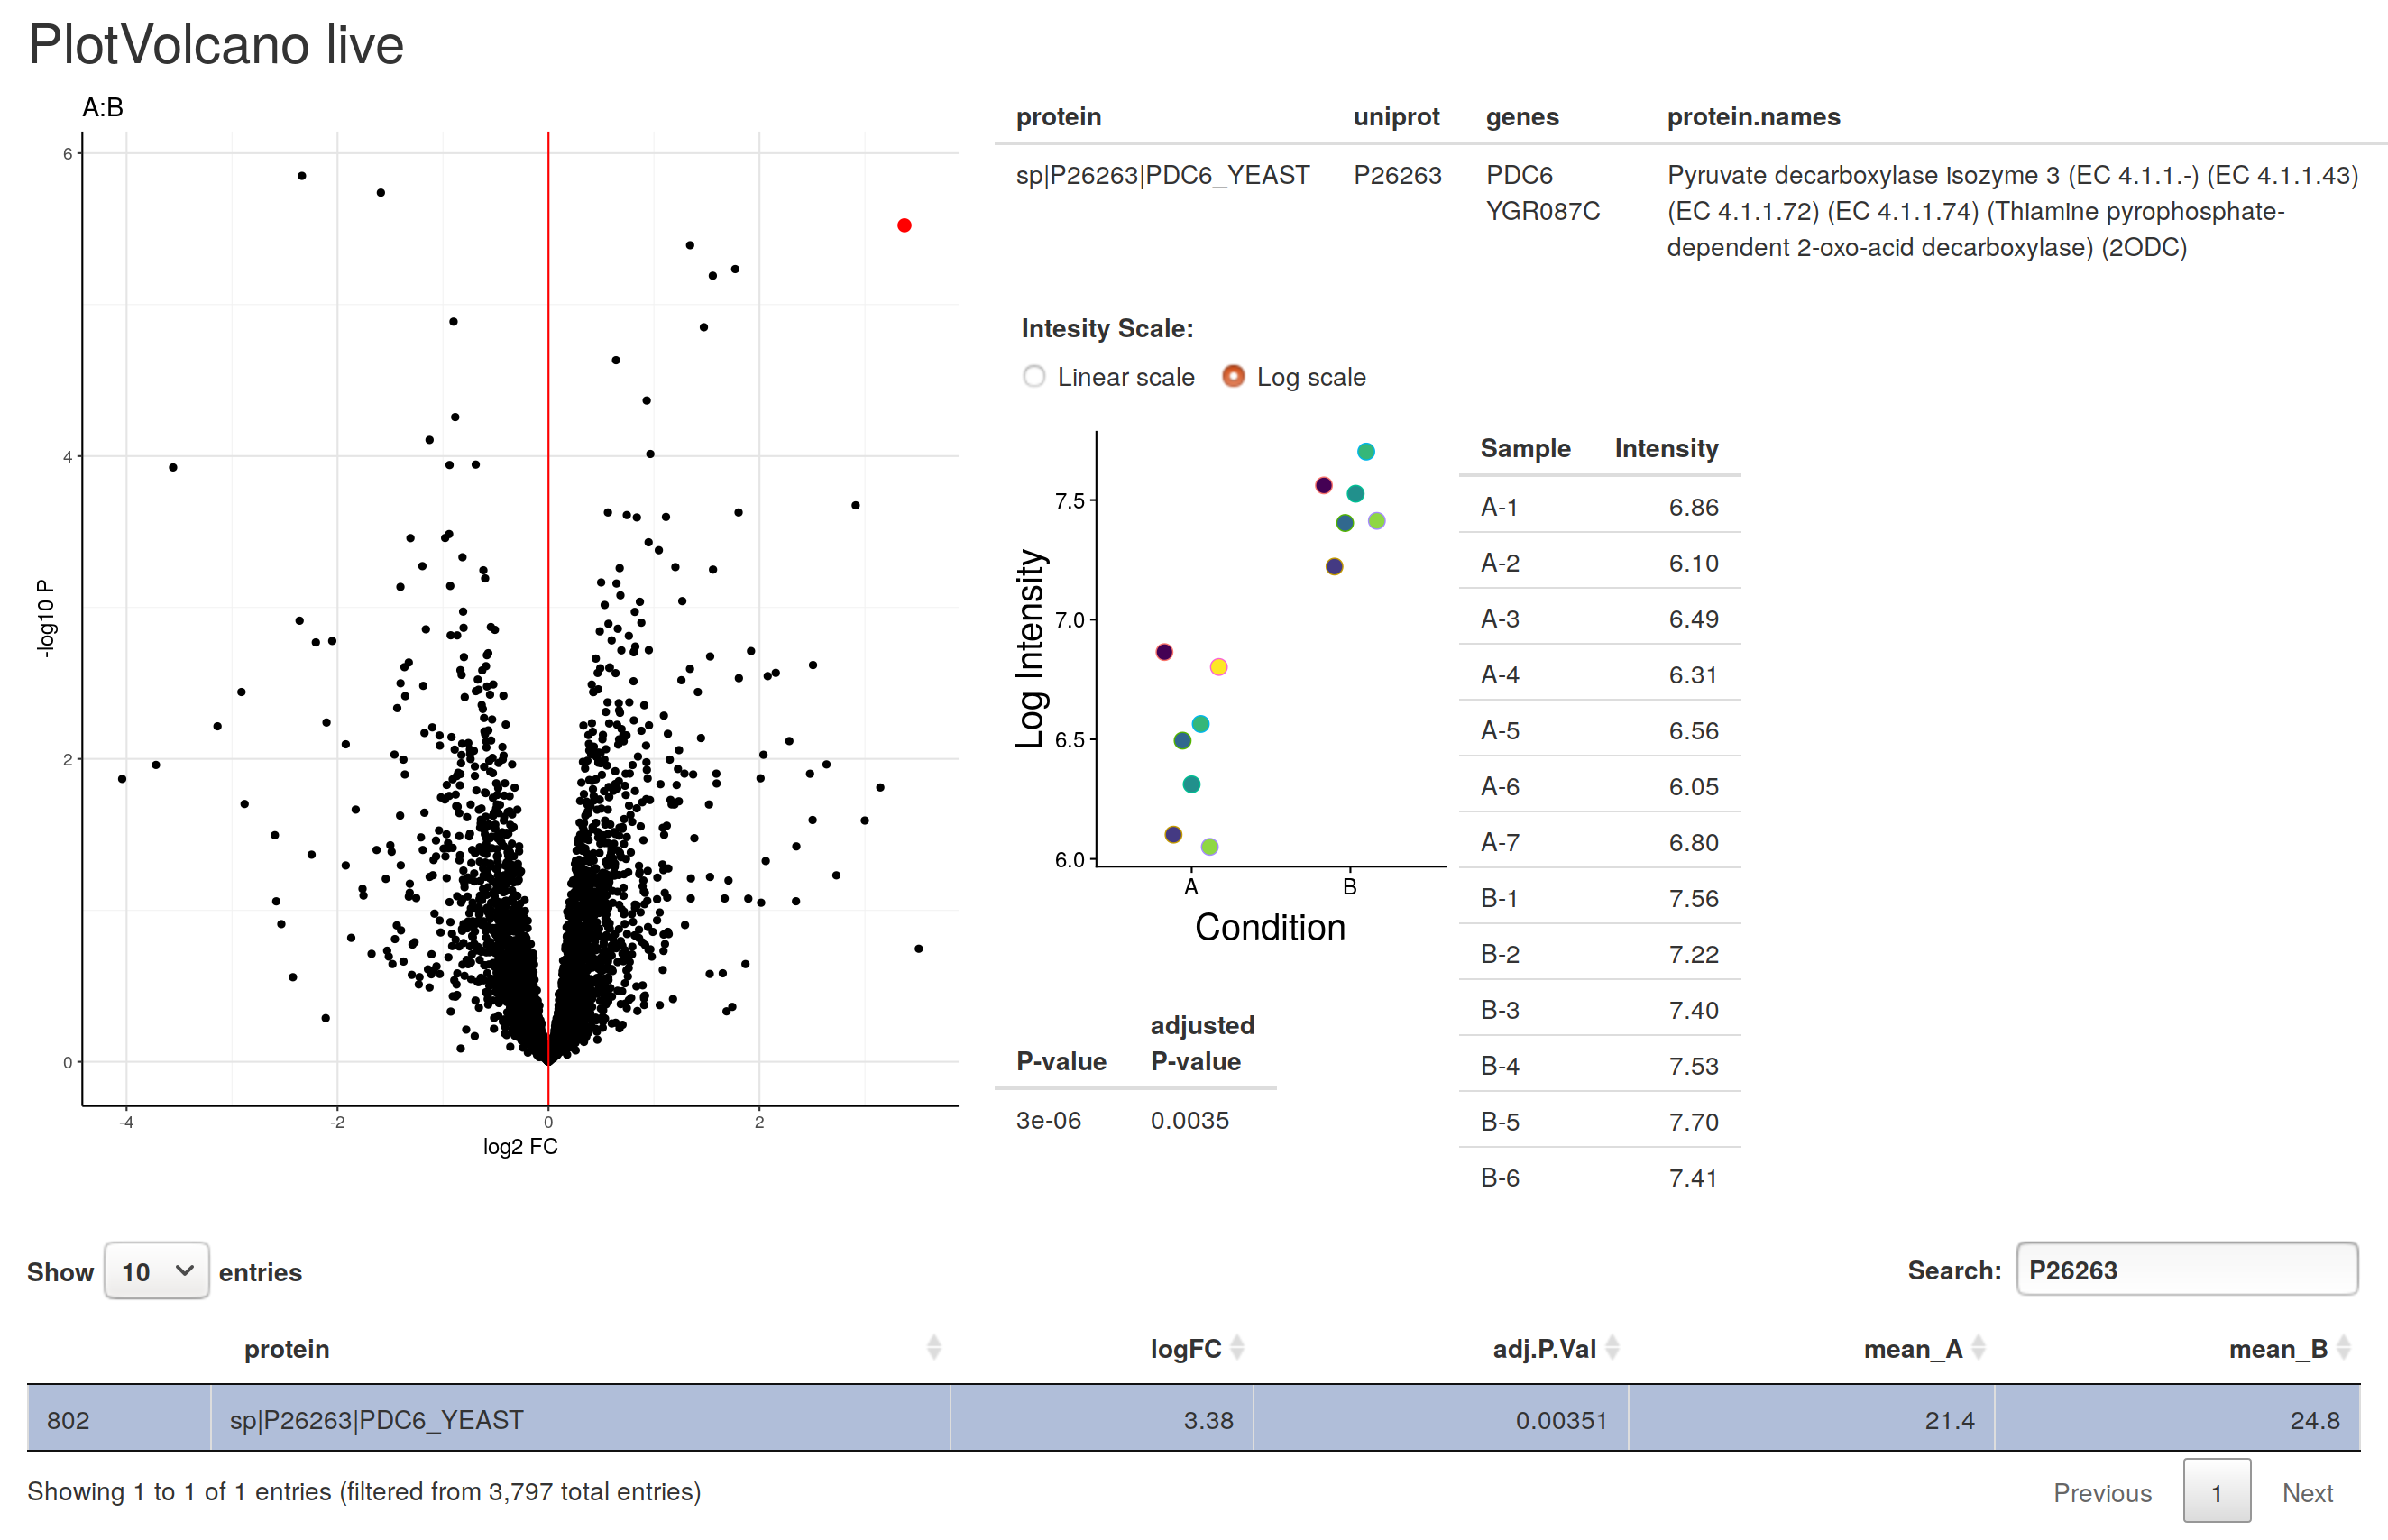
\includegraphics{../volcano_live_screenshot} 

}

\caption{\label{fig:shiny}A screenshot of the interactive data explorer in Proteus, using the Shiny framework. It shows an interactive volcano plot with a selected protein marked in red. The user can select proteins from the plot by hovering the mouse over a dot representing one protein. To the right, there are protein annotation, intensity plot, detailed intensity table and a p-value from the differential expression test. At the bottom there is a row selected from the full table of proteins by typing the protein ID in the search box.}\label{fig:fig_shiny}
\end{figure}

\subsection{Minimal example}\label{minimal-example}

A basic data processing flow in \emph{Proteus} is a follows: read the
evidence data and metadata, aggregate peptides and proteins, normalize
protein data, perform differential expression and explore the results.
Assuming that R variables \texttt{evidenceFile} and
\texttt{metadataFile} point to \emph{MaxQuant's} evidence file and a
small text file describing the design of the experiment (that is how
samples and conditions relate to evidence data) the minimal R code to
process these data is:

\begin{verbatim}
# read evidence data
evidence <- readEvidenceFile(evidenceFile)

# read metadata
metadata <- read.delim(metadataFile, header=TRUE, sep="\t")

# aggregate peptides
peptides <- makePeptideTable(evidence, metadata)

# aggregate proteins
proteins <- makeProteinTable(peptides)

# normalize protein intensities
proteins <- normalizeData(proteins)

# differential expression
res <- limmaDE(proteins)

# interactive data expolorer
plotVolcano_live(proteins, res)
\end{verbatim}

Here we used default parameters in all steps, but each function has
several parameters allowing the full control over, e.g., the way
peptides and proteins are aggregated or normalized. \emph{Proteus} comes
with a set of tutorials (R vignettes) using real data examples to
illustrate every step of data processing. Each function in the package
is accompanied with detailed documentation and examples.

\section{Proteus vs Perseus}\label{proteus-vs-perseus}

Here we compare performance of \emph{Proteus} (version 0.2.8) to
\emph{Perseus} (version 1.6.1.3), a commonly used \emph{MaxQuant} data
analysis tool with a graphical user interface, available for MS Windows,
on two examples. First, we analyse a label-free proteomics data set in
two conditions and three replicates each. Second, we create a simulated
data set based on a large real data set to investigate power and false
positives from both tools. We focus on the performance of the
differential expression, which is carried out by a t-test in
\emph{Perseus} and \emph{limma} in \emph{Proteus}.

\subsection{Simple data set}\label{simple-data-set}

First we compared differential expression offered by both packages using
the same protein data set. We used a subset of a large data set from
Gierlinski et al. (in preparation). We read the evidence file and
filtered out reverse sequences and contaminants. Then, we created
peptide table based on three randomly selected replicates in each
condition (samples Mut-7, Mut-28, Mut-34, WT-8, WT-13, WT-25). Peptides
were aggregated by summing multiple evidence entries for a given
(unmodified) sequence. Next, we aggregated peptides into proteins using
the high-flyer method and peptide-to-protein mapping based on the
`leading razor protein' column from evidence data. We filtered protein
intensities in these replicates, so at least one data point was present
in each condition. These data were normalized to median (that is, after
normalization median intensity in each sample was the same). The
resulting intensity table containing 3338 proteins in two conditions in
three replicates each was processed in \emph{Perseus} and
\emph{Proteus}.

In \emph{Perseus} we \(\log_2\)-transformed these data and filled
missing values with random imputation, using the default parameters,
width = 0.3 and down shift = 1.8. Then, we performed a two-sample
\(t\)-test and exported the results as a generic table. In
\emph{Proteus} we \(\log_2\)-transformed data and performed differential
expression using \emph{limma}. Since the protein intensities were the
same, we compared the difference between \(t\)-test with imputation
versus \emph{limma} without imputation.

\begin{figure}[H]

{\centering \includegraphics{proteus_files/figure-latex/fig_perseus_limma-1} 

}

\caption{\label{fig:perseus_limma}Perseus vs limma for a selection of 3 vs 3 replicates. A. P-value (not adjusted) comparison. B. Number of significant proteins. C. Volcano plot using fold-change and p-values from Perseus. All data are in yellow background. The limma-significant-only proteins are as blue circles, the perseus-significant-only proteins are as green triangles. Proteins significant in both tools are as pink diamonds. D. Volcano plot using fold-change and p-values from Proteus. Symbols are the same as in C.}\label{fig:fig_perseus_limma}
\end{figure}

Figure \ref{fig:perseus_limma} shows the comparison of p-values,
significantly differentially expressed proteins and volcano plots for
both approaches. There were 39 proteins called as significant by both
methods, 15 only by \emph{Perseus} and 45 only by \emph{limma} (in
\emph{Proteus}). We can see in Figure \ref{fig:perseus_limma}C a small
group of proteins called by \emph{limma} only where \emph{Perseus}
reported large p-values (6 blue circles at the bottom of the plot).
These proteins have missing data and rather large intensity. Imputation
in \emph{Perseus} filled the missing values with low intensities,
inflating variance and missing what otherwise would be differentially
expressed. An example of such a protein is shown in Figure
\ref{fig:protein_examples}A. Another group of \emph{limma}-only blue
circles in Figure \ref{fig:perseus_limma}C indicates that the
permutation FDR method used in \emph{Perseus} is slightly more
conservative that that in \emph{limma}. All these proteins have adjusted
p-values near the limit 0.05. An example of such protein is shown in
Figure \ref{fig:protein_examples}B. The proteins plotted as green
triangles (see Figure \ref{fig:perseus_limma} C and D) are marked as
differentially expressed by \emph{Perseus} but not \emph{limma}. They
typically have small variance and small fold change. They are called
significant by a simple t-test but not by \emph{limma}, which moderates
variance and avoids cases of unusually small variability. An example of
such protein is shown in Figure \ref{fig:protein_examples}C. We note
that these data can be easily eliminated from \emph{Perseus} by setting
a fold-change limit in a \(t\)-test.

\begin{figure}[H]

{\centering \includegraphics{proteus_files/figure-latex/protein_examples-1} 

}

\caption{\label{fig:protein_examples}Selected examples of proteins called as significant by one tool only. UniProt identifiers are shown on top of each panel. A. Called by limma only. Imputation in Perseus inflated variance creating a false negative. B. Called by limma only. Perseus FDR is more conservative than that in limma at the same limit of 0.05. C. Called by Perseus only. An example of very low variance, which is moderated and called negative by limma. Data imputed by Perseus are marked with open circles.}\label{fig:protein_examples}
\end{figure}

The imputation in \emph{Perseus} is designed to fill missing
low-intensity data with a randomly generated Gaussian numbers (see
supplemental figure 3 in \citet{tyanova2016}). However, on some
occasions a datum can be missing even at high intensities. In such cases
variance is dramatically inflated and the protein is not called as
differentially expressed. We warn against using data imputation.
\emph{limma} offers a better approach to missing data, by modelling
mean-intensity variance and using moderated variance for the test.
Certainly, the imputation step can be omitted in \emph{Perseus}, but
this reduces power and rejects data with only one replicate available in
a condition. Again, \emph{limma} can estimate variance and make a
decision about differential expression even in such extreme cases (at an
increased risk of a false positive).

\subsection{Simulated data}\label{simulated-data}

Next, we compared performance of differential expression in both tools
using simulated data. We generated a simulated set based on real data.
Since we have a good data set of two conditions in 35 replicates each
(Gierlinski at al. in preparation), we used it to find the mean-variance
relationship and the rate of missing values as a function of the
intensity.

Figure \ref{fig:full_data_stats}A shows the relation between the
logarithm of the variance and logarithm of the mean calculated across
all 35 replicates (data from both conditions aggregated). It is well
approximated by a straight line. Figure \ref{fig:full_data_stats}B shows
the distribution of the number of ``good'' replicates as a function of
the logarithm of the mean intensity. The good replicates are those with
signal detection, as opposed to missing data. We see that in our data
set all measurements with \(\log_2\) mean below \textasciitilde{}19
contain only one good replicate (out of 35!).

\begin{figure}[H]

{\centering \includegraphics{proteus_files/figure-latex/lfq_stats_plots-1} 

}

\caption{\label{fig:full_data_stats}Properties of the full data set with 35 replicates in two conditions. A. Logarithm of the variance versus logarithm of the mean is very well approximated by a linear function. B. Number of good replicates as a function of the loarithm of the mean intensity (that is not missing data). Data from both conditions were aggregated.}\label{fig:lfq_stats_plots}
\end{figure}

We used this information to create a simulated data set. We generated
data in two conditions in three replicates each and allowed for missing
data in each condition. We chose 7 values of \(\log_2 M\) (mean) between
17 and 29 and 15 values of \(\log_2 FC\) (fold change) between 0 and
2.8. For each combination of \(\log_2 M\) and \(\log_2 FC\) we generated
two random samples of up to 3 data points from the log-normal
distribution with the given mean and variance estimated from the linear
function found from real data. The first sample had the mean \(M\), the
second sample had the mean \(M * FC\). For each sample the number of
good replicates was generated based on data in Figure
\ref{fig:full_data_stats}B. First, for the given \(M\), we used the
cumulative distribution of the number of good replicates to generate a
number between 1 and 35. This was then sub-sampled to the 3 replicates
generated (for example, if 10 was generated in the first step, we
created a vector of 10 good and 25 bad replicates and drew a random
sample of 3). Since we are not interested in samples with no data, we
enforced at least one good replicate in each sample. This means that
data with only one good replicate will be over-represented for very low
intensities. This is not an issue as our aim is to assess tool
performance at each intensity level and low intensities will invariably
contain a lot of missing data. For each combination of \(\log_2 M\) and
\(\log_2 FC\) we generated 1000 samples in two conditions, using this
technique. This gave us a large set of 105,500 ``proteins'' covering a
wide range of intensities and fold changes.

\begin{figure}[H]

{\centering \includegraphics{proteus_files/figure-latex/plot_sim_limma-1} 

}

\caption{\label{fig:simulation_rates}Results for the full set of simulated data with 3 replicates. Top panels show limma, bottom panles show Perseus results. A and C show the proportion of tests called as signficant as a function of the simulated fold change (FC) and mean (M). B and D show the false discovery rate, that is the proportion of tests for simulated log FC = 0 called as significant.}\label{fig:plot_sim_limma}
\end{figure}

We performed differential expression on the simulated data using
\emph{Perseus} and \emph{Proteus}. In \emph{Perseus} we imported
simulated data from a file, \(\log_2\)-transformed, applied default
imputation and used a two-sample \(t\)-test. In \emph{Proteus} we
\(\log_2\)-transformed the data and used \emph{limma} for differential
expression. The results are shown in Figure \ref{fig:simulation_rates}.
Panels A and C show the proportion of proteins called significant in a
group of 1000 proteins for each combination of fold change and mean
intensity. We can see that \emph{limma} (in \emph{Proteus}) performs
well across all intensities, discovering almost all positives for the
highest \(\log_2 FC = 2.8\) used here. In contrast, the sensitivity of
\emph{Perseus} drops dramatically at low intensities. Even at medium
intensities of \(\log_2 M = 23\) only about half of the changing
proteins are discovered at large fold changes of \(\log_2 FC = 2\). See
also Figure \ref{fig:significant_proportion_comparison}A.

The main reason for this behaviour is imputation of missing replicates
in \emph{Perseus}. We notice that due to the way simulated data were
generated, all proteins for the lowest intensity \(\log_2 M = 17\)
contain only one good replicate in each condition. As the \(t\)-test
cannot deal with samples of one, imputation is necessary and the result
is randomized. On the other hand, \emph{limma} borrows information
across the entire set and builds a reliable model of variance which
works for any sample size. As we can see from the bottom curve in Figure
\ref{fig:simulation_rates}A (corresponding to \(\log_2 M = 17\))
\emph{limma} performs well even in tests of one versus one replicate.

The price to pay for increased sensitivity of \emph{limma} is the
increased false discovery rate (FDR). We can estimate FDR as a
proportion of proteins called significant at \(\log_2 FC = 0\). Figure
\ref{fig:simulation_rates}B shows that FDR for \emph{limma} exceeds the
assumed limit of 0.05 at the three lowest intensities. \emph{Perseus}
discovers far fewer positives at these intensities, which results in
lower FDR (Figure \ref{fig:simulation_rates}D).

\begin{figure}[H]

{\centering \includegraphics{proteus_files/figure-latex/plot_sim_limma_n2-1} 

}

\caption{\label{fig:simulation_filt_rates}Results for the filtered set of simulated data with 3 replicates. Only data with at least 2 replicates in each condition were used. Panels are the same as in Figure \ref{fig:simulation_rates}.}\label{fig:plot_sim_limma_n2}
\end{figure}

Since imputation is clearly an issue we decided to compare
\emph{Proteus} and \emph{Perseus} using data that do not require
imputation. We used the same simulated data set, but filtered out all
proteins with only one good replicate in either condition. Filtering
low-replicate data would reflect a more realistic workflow for a
researcher who doesn't want to apply imputation. After filtering we
processed data in \emph{Perseus} and \emph{Proteus} as before, but
skipped the imputation step in \emph{Perseus}. Results are shown in
Figure \ref{fig:simulation_filt_rates}. Not surprisingly, the
significant proportion of \emph{limma} and \emph{Perseus} are now more
similar, though \emph{limma} still offers slight advantage (see also
Figure \ref{fig:significant_proportion_comparison}B). The false
discovery rate is now better controlled by \emph{limma} than by
\emph{Perseus} where 4 out of 5 intensity groups result in
\(FDR \sim 0.1\).

\begin{figure}[H]

{\centering \includegraphics{proteus_files/figure-latex/compare_significance_23-1} 

}

\caption{\label{fig:significant_proportion_comparison}Comparison of significance curves corresponding to log M = 23. A. Full simulatred data set (see Figs. \ref{fig:simulation_rates}A and  \ref{fig:simulation_rates}C). B. Filtered simulated set (see Figs. \ref{fig:simulation_filt_rates}A and \ref{fig:simulation_filt_rates}C). Perseus results are shown in dahsed curves, Proteus results are represented by solid curves.}\label{fig:compare_significance_23}
\end{figure}

\section{Conclusions}\label{conclusions}

R is becoming one of the most widely used tools for data science and
statistical computing, in particular in academia
\citep{tippmann2014, muenchen2017}. Its strenght is built on the wealth
of statistical libraries available. \emph{Proteus} adds to a rapidly
growing suite of bioinformatics packages in R. It not only performs
specific tasks related to processing of \emph{MaxQuant} output, but
opens peptide and protein data to further analysis and visualisation. It
offers an alternative to a popular package \emph{Perseus} for
researchers willing to use R.

R is a scripting language and when data and code are published together,
it makes data processing fully reproducible. Any analysis performed in
\emph{Proteus} can be replicated by any researcher, including all
intermediate steps, simply by running the original code again. We
recommend using the \emph{RStudio} environment \citep{rstudio}, where
the code can be executed step-by-step and each R object can be easily
scrutinised. R is a cross-platform project and can be used on most
operating systems. Needless to say, \emph{Proteus} is fully open source.

\emph{Proteus} uses a powerful package \emph{limma} for differential
expression analysis, allowing for stable analysis of data with missing
values, common in label-free MS proteomics, with no need for random
imputation. Instead, \emph{limma} borrows information between
peptides/proteins to build a robust model of variance and performs
differential expression tests based on this model. We demostrate that
this offers a clear advantage in terms of sensitivity over a \(t\)-test
combined with random imputation. This makes \emph{Proteus} particularly
useful for label-free data with a small number of replicates.

\section{Acknolwdgments}\label{acknolwdgments}

The authors would like to thank Katharina Trunk, Sarah Coulthurst and
Julien Peltier for kindly providing example data used in \emph{Proteus}
package and in this paper.

\renewcommand\refname{References}
\bibliography{proteus.bib}


\end{document}
